\documentclass[]{article}
\usepackage[utf8]{inputenc}
\usepackage{amsfonts} 
\usepackage{graphics}
\usepackage{listings}
\usepackage{xcolor}
\usepackage{amsmath}
\usepackage{tikz}
\usepackage{hyperref}
\usepackage{float}
\usepackage[linesnumbered,ruled,vlined]{algorithm2e}
\usepackage{changepage}
\usepackage{amsmath}
\usepackage[backend=biber, style=numeric]{biblatex}

\addbibresource{references.bib}

\definecolor{codegreen}{rgb}{0,0.6,0}
\definecolor{codegray}{rgb}{0.5,0.5,0.5}
\definecolor{codepurple}{rgb}{0.58,0,0.82}
\definecolor{backcolour}{rgb}{0.95,0.95,0.92}

\lstdefinestyle{mystyle}{
    backgroundcolor=\color{backcolour},   
    commentstyle=\color{codegreen},
    keywordstyle=\color{magenta},
    numberstyle=\tiny\color{codegray},
    stringstyle=\color{codepurple},
    basicstyle=\ttfamily\footnotesize,
    breakatwhitespace=false,         
    breaklines=true,                 
    captionpos=b,                    
    keepspaces=true,                 
    numbers=left,                    
    numbersep=5pt,                  
    showspaces=false,                
    showstringspaces=false,
    showtabs=false,                  
    tabsize=2
}

\lstset{style=mystyle}

\title{Optimisation Multicritères:\\
        Voyageurs de commerce bi-critères: Coûts/Durée}
\author{Valentin Hesters 20201346}
\date{19 Novembre 2024}



\begin{document}
\maketitle
\renewcommand*{\contentsname}{Sommaire}
\tableofcontents
\vspace{0.75cm}
le dossier du code se trouve à cette adresse :\\
\href{https://github.com/suprawall/MTSP}{https://github.com/suprawall/MTSP}\\

Pour lancer le code il s'uffit d'executer \textit{main.py}\\
la variable globale NB\_BLOCKS
gère la taille du graph.

\section{Implémentation}
    \subsection{Génération du graphe}
        Un seul type de graphe est considéré dans cette implémentation:
        le graphe en blocs. Le code source se trouve dans le fichier
        \textit{graph\_init.py}. Le graphe se compose d'un bloc initiale de 4 noeuds
        reliés par 6 arrêtes. Les blocs suivants sont ajoutés à la 
        "droite" de celui-ci, ils se composent de 2 noeuds et 4 arrêtes.
        La taille du graphe généré est définie par la variable globale
        NB\_BLOCKS dans le fichier \textit{main.py}. Ainsi, chaque graphe
        considéré dispose de:\\
        $4 + 2 * (NB\_BLOCKS - 1)$ noeuds, et $6 + 4 * (NB\_BLOCKS - 1)$ arcs.\\
        Le chemin a minimiser est celui entre le premier noeud
        et l'avant dernier.
        \begin{figure}[H]
            \centering
            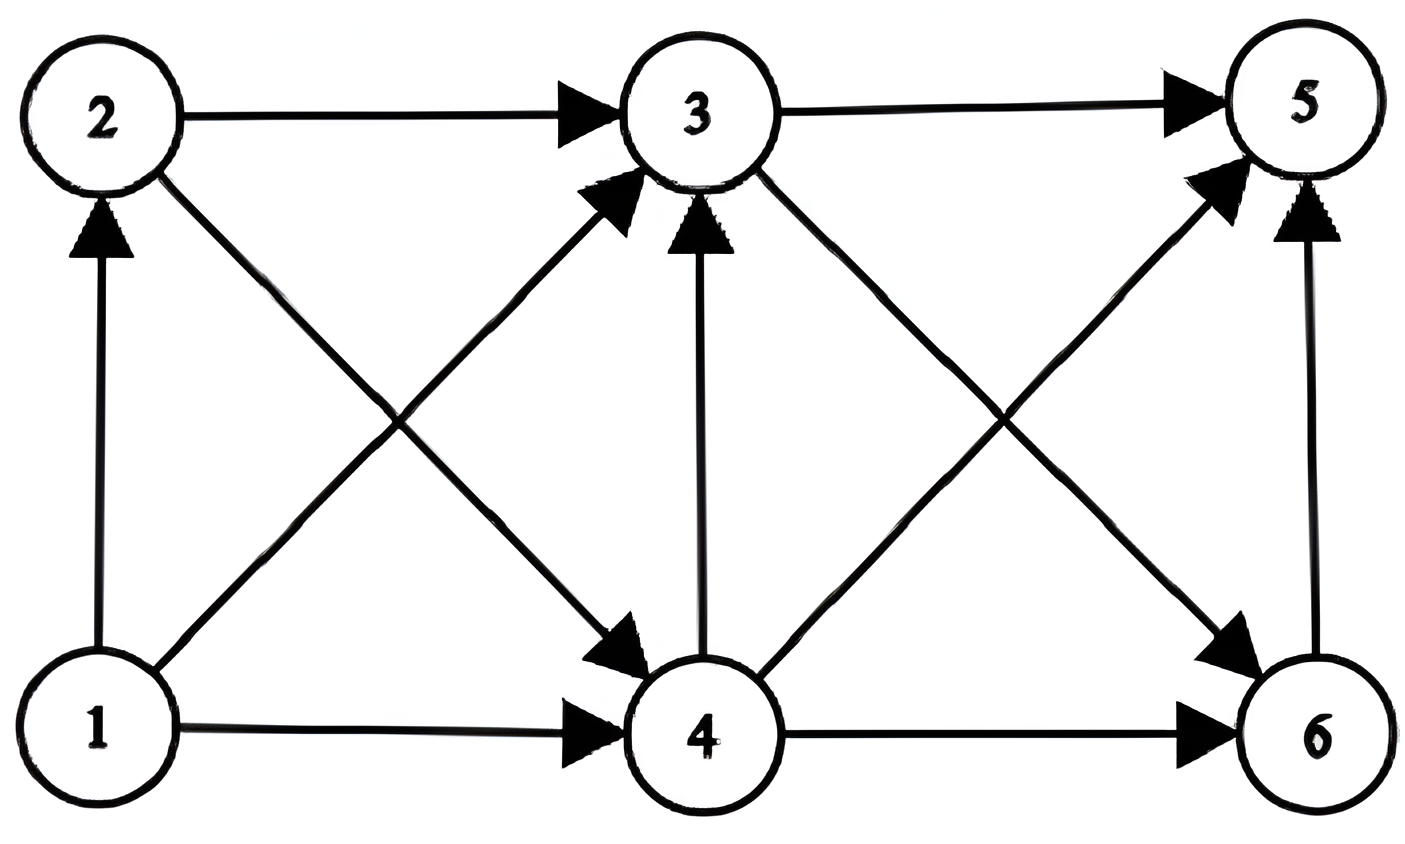
\includegraphics[width=0.5\textwidth]{output/pixelcut-export.png}
            \caption{\textit{graphe en block: chemin entre 1 et 5}}
        \end{figure}

        les poids sont ajoutés à chaque arcs sous forme de tuple (coût, durée). 
        L'intervalle de valeurs pour chacun des critères est définie par deux variable
        global dans main.py. Dans la partie expérimentale de ce rapport, chaque coût
        et chaque durée est compris entre 1 et 20. Pour avoir une distinction nette entre
        des chemins efficaces pour minimiser le coût et d'autres pour minimiser la durée,
        les poids sont répartis comme ceci: pour chaque arcs on choisit au hasard
        entre le coût et la durée. Si le coût a été choisi alors il aura une valeur
        aléatoire entre 1 et le plafond (ici 20), et la durée aura une valeur aléatoire
        entre 1 et le plafond/3 (ici 20/3 arrondi à 6). Ainsi la durée a plus de chance 
        d'être bien inférieur au coût, mais la probabilité n'est pas de 0 non plus, ce qui
        assure une distribution plus au moins naturelle dans le graphe tout en étant assuré
        d'avoir une distinction entre les solutions qui minimise le coût et les solutions qui
        minimise la durée sur des grands graphes.

        \subsection{pseudo-code}
        
        Le code pour effectuer l'algorithme epsilon contrainte via la relaxation
        lagrangienne se trouve dans le fichier \textit{execute\_lagrangienne.py}.
        Dans un premier, on cherche à trouver la solution qui minimise le coût et
        celle qui minimise la durée. Pour ce faire on utilise le solveur python
        Pupl \url{https://coin-or.github.io/pulp/}. La fonction: "def solveur(G, weights, critere):"
        du fichier \textit{execute\_brutforce.py} permet de spécifier quel critère on 
        souhaite minimiser (0 pour le coût et 1 pour la durée). On associe à chaque arcs
        une variable binaire pour savoir si l'arc est gardé dans la solution. On l'a
        multiplie avec le poid de cet arc sur le critère concerné. Ensuite on définie le 
        faite que: le noeud source doit avoir un flux sortant de 1, le noeud cible un flux
        entrant de 1 et que chaque noeud doit avoir un flux entrant et sortant égal.\\
        Ensuite on récupère le couple de poid associé à la solution via la fonction
        "get\_weight\_path" à la ligne 23. La premiere contrainte est donc la durée de
        la solution qui minimise le coût. A partir de là on peut lancer l'algorithme.\\
        \\
        le code principal se trouve dans la fonction "execute\_lagrangienne" à la ligne
        114 de \textit{execute\_lagrangienne.py}. Il se compose de 2 boucles: une pour 
        epsilon contrainte et une pour la relaxation lagrangienne.\\
        
        \begin{enumerate}
            \item On initialise un tableau de parametre contenant des tuples: (coût, durée - contrainte epsilon), pour toutes les solutions de la frontière de Pareto.
            \item On calcule les fonctions de lagrange de chaqu'un des élements dans le tableau paramètre
            \item On trouve le $\lambda$ qui maximise les minimums des fonctions dans le tableau paramètre.
            \item On calcule les nouveaux poids pour chaque arcs (coût + $\lambda$ * durée), et on cherche la solution optimale à ce problème mono-critère via le solveur Pulp.
            \item On l'ajoute au tableau paramètre et on boucle depuis l'étape 2 jusqu'à convergence
            \item Une fois sortis de cette boucle on prend la dernière solution on l'ajoute à la frontiere de Pareto et on définie la prochaine contrainte epsilon comme étant la durée de cette solution
            \item On boucle depuis l'étape 1 jusqu'à ce que la durée de la solution trouvée soit égale à la durée de la solution qui minimise la durée 
        \end{enumerate}

        Le dossier se compose aussi d'un fichier \textit{execute\_brutforce.py}, qui
        permet d'executer la méthode epsilon-contrainte de manière brut force, c'est 
        à dire qu'à chaque itération on trouve la nouvelle solution via le solveur Pulp
        directement. On utilise cette fois la fonction "solveur\_containte" de la ligne 73
        pour chercher le chemin qui minimise le coût tout en ayant une contrainte sur la 
        durée. J'ai implémenté cette méthode, qui donne donc un ensemble complet Pareto optimale,
        pour pouvoir la comparer avec les résultats obtenus via l'algorithme.

        \section{Résultats expérimentaux}

        Le graphique le plus intéressant est celui qui compare les frontières de Pareto
        obtenue via l'algorithme lagrangien et via brutforce. Voici en exemple sur un petit
        graphe de 30 blocs, pour que tous les points du brutforce soit encore distinguables.
        
        \begin{figure}[H]
            \centering
            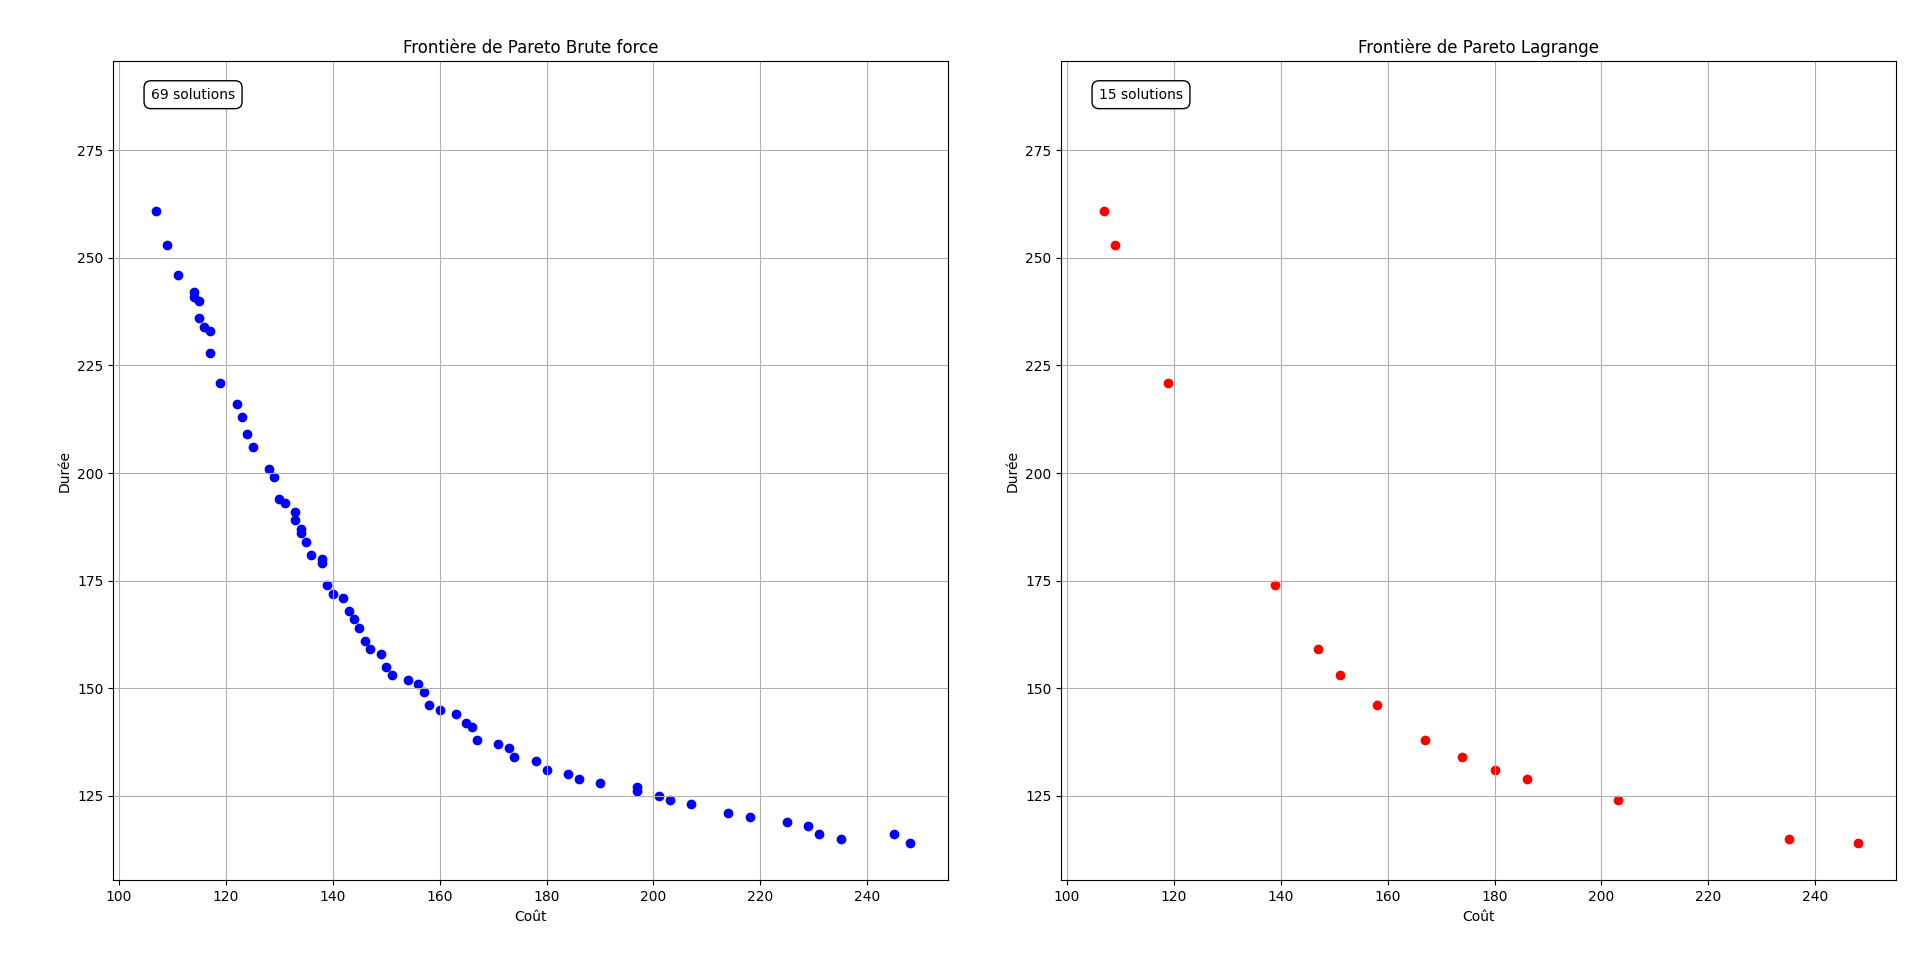
\includegraphics[width=1.25\textwidth]{Résultats/comparaison/30 blocks.png}
            \caption{\textit{comparaison sur 30 blocs}}
        \end{figure}

        \begin{figure}[H]
            \hspace{-2cm}
            \centering
            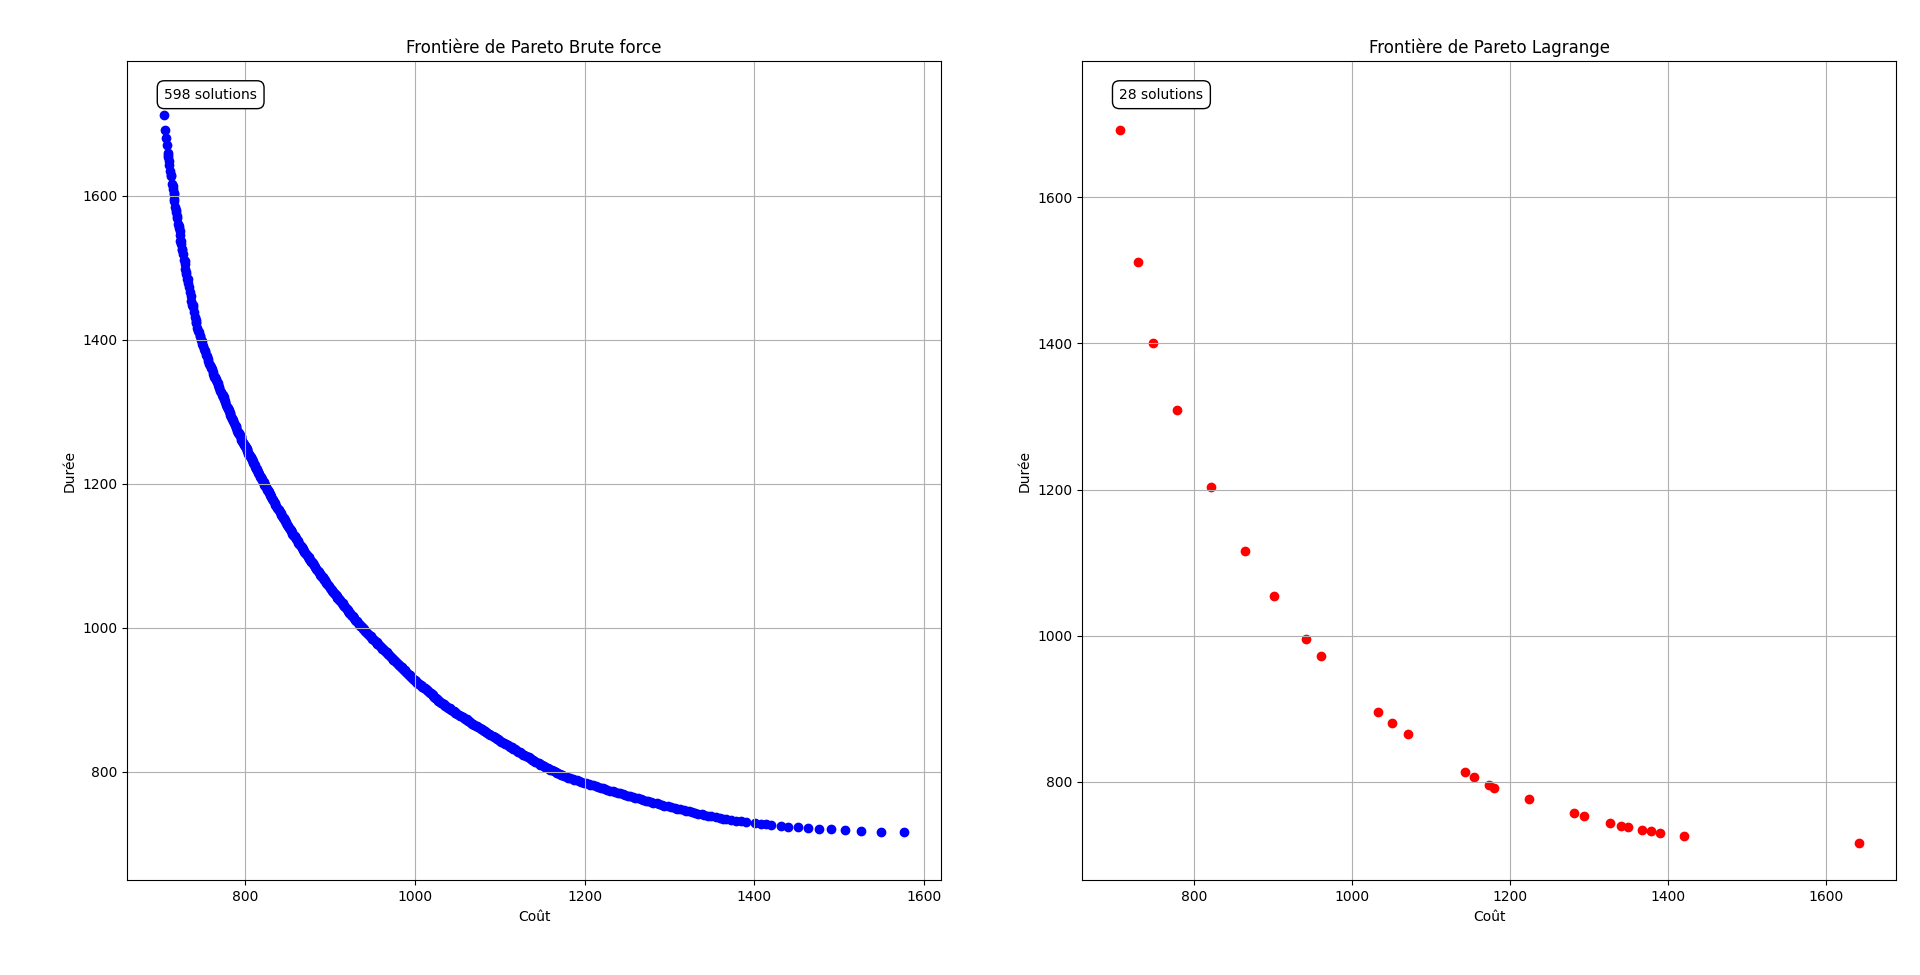
\includegraphics[width=1.25\textwidth]{Résultats/comparaison/200.png}
            \caption{\textit{comparaison sur 200 blocs}}
        \end{figure}

        On remarque que les solutions obtenues via l'algorithme ont tendance à être plus
        concentré vers la fin de la courbe plutôt qu'au début.

        \begin{figure}[H]
            \centering
            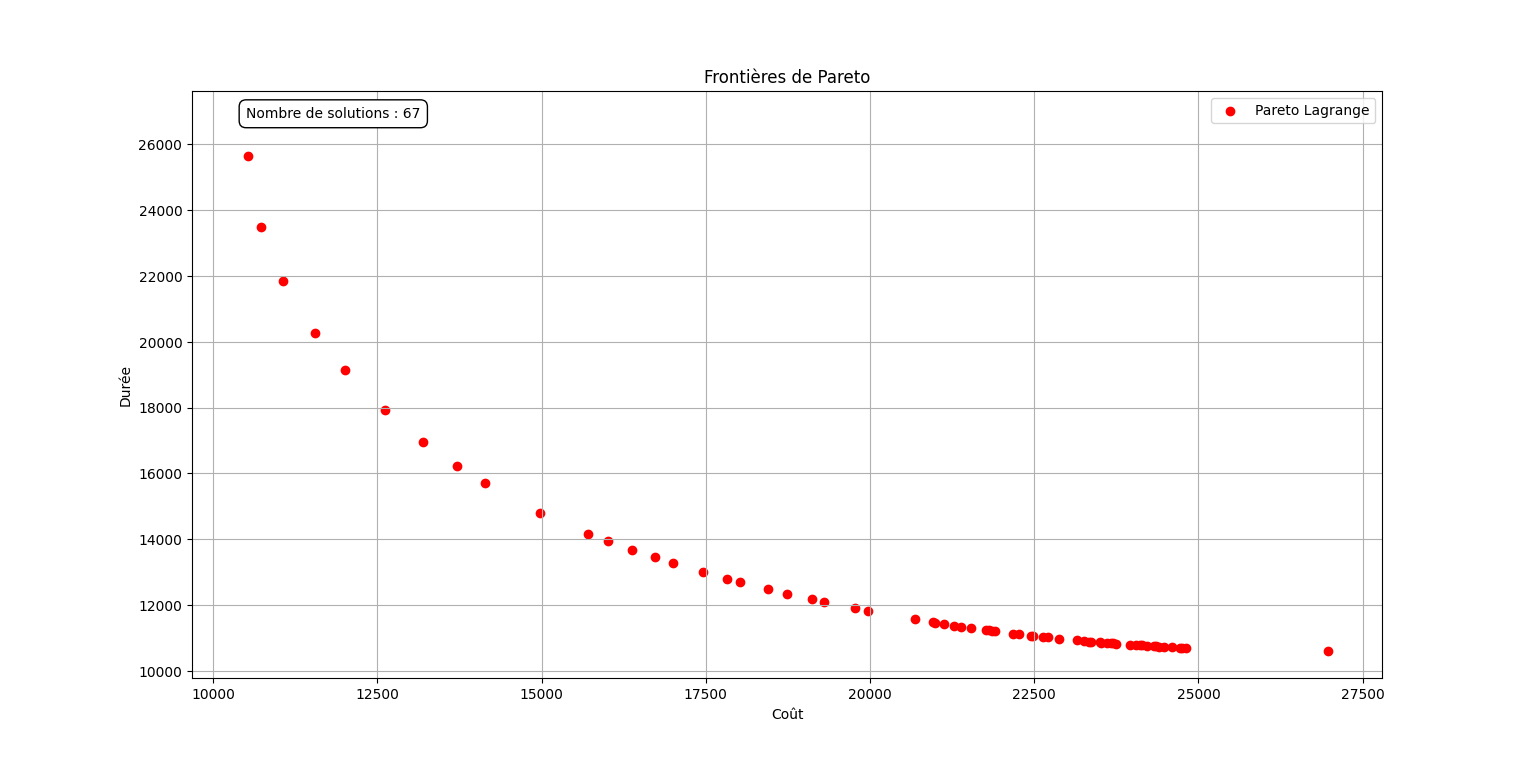
\includegraphics[width=1\textwidth]{Résultats/pareto lagrange 3000 blocks.png}
            \caption{\textit{3000 blocs: 12 002 arcs}}
        \end{figure}


        \begin{figure}[H]
            \centering
            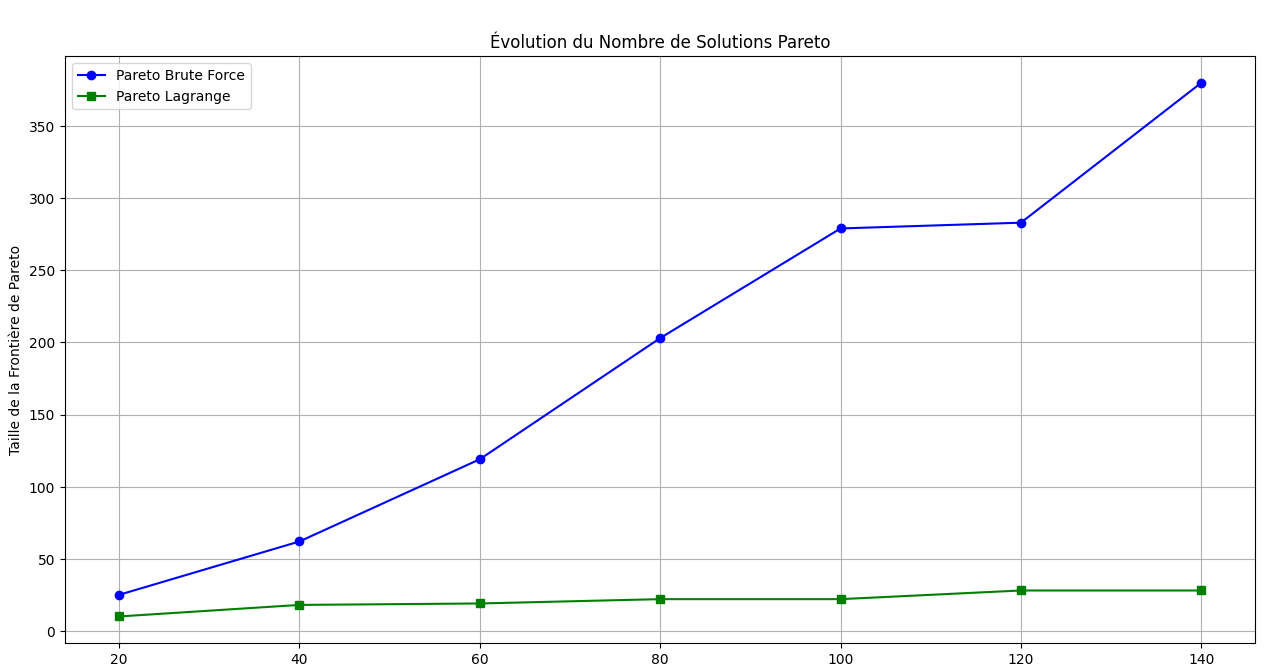
\includegraphics[width=1.1\textwidth]{output/lagrange 10 28 brute force 25 380.png}
            \caption{\textit{comparaison nombre de solutions}}
        \end{figure}




        


\end{document}